% !TEX root = Tesi.tex
\chead{}
\chapter{Background}

\section{The Internet of Things and the Web}
\label{section:iot}
During the last few years, and in an increasing manner, we have been standing at the forefront of a world where virtually everything can be connected directly to the Internet. This has resulted in an increasingly connected world where emerging technologies enable objects to be linked among themselves through the use of new devices and sensors.

This new era of the Internet has become visible in our everyday lives: from souped-up gadgets tracking our every move to environments capable of predicting our actions and emotions, the list keeps growing every day.

The Internet, consisting of things, rather than just computers, is becoming more central to society than the web as we once knew it. This does not necessarily mean that the traditional web is expected to die, but rather that its role will be reduced to that of a language used for displaying content on devices which are supposed to be more ubiquitous but are not as necessary.

The first “pioneer species” within this ecosystem of "invisible buttons" has certainly been the smartphone. Its increasing usage among the masses has made it the perfect catalyst for such a revolutionary change. One of the many uses that has helped us better understand this pioneering technology is the way that it beams information about our location and speed when we take it with us in a car resulting in a real-time traffic information accessible by everyone. In such a scenario, the actual gathering of real traffic data happens without the user ever knowing of the data transmission and without a need for interaction such as a click on a button or navigating to a particular web page.

This sort of awareness, especially as it relates to the physical world, leads to areas in space that are listening to the environment and triggering events depending on certain conditions in an entirely automatic way, like a smartphone getting into the range. There are currently applications in which the smartphone can be placed as close as two centimeters away from the top of a credit card reader to enable touch payments, or where the smartphone is detected in a large space, such as a room, triggering an event indicating that a user has entered or exited so that the lights can bed switched on or off.

It is important to differentiate these interconnected objects from being simple on-off switches; they would not be very useful if this was the case. However, because the possible actions they can trigger can be affected by an endless list of other variables such as the time of the day, our personal preferences or the actions of others, they can quickly be scaled to reate a better program that creates more efficient interactions in our physical world.

Leveraging the use of a smartphone acting as a proximity sensor is just an artifact of the current state of technology. The same result could be accomplished with any number of sensors directly connected to the Internet so long as those sensors are capable of dealing with motion, sound, light temperature, humidity, and other variables.

Companies like Apple have been embracing the idea of invisible buttons since the beginning of this new era of sensors and devices. 

While the company has been embracing the technology by foreseeing its potential from the beginning, it recently rolled out a new line of devices called iBeacon.

In a nutshell, the iBeacon allows any newer iPhone or Android phone to know its position in space with centimeter precision. Similarly to a more precise Global Positioning System (GPS) that works indoors, an iBeacon allows the developers to take advantage of the technology to define “invisible buttons” of just about any dimension.

\vspace{0.5cm}
\begin{figure}[htbp]
  \centering
    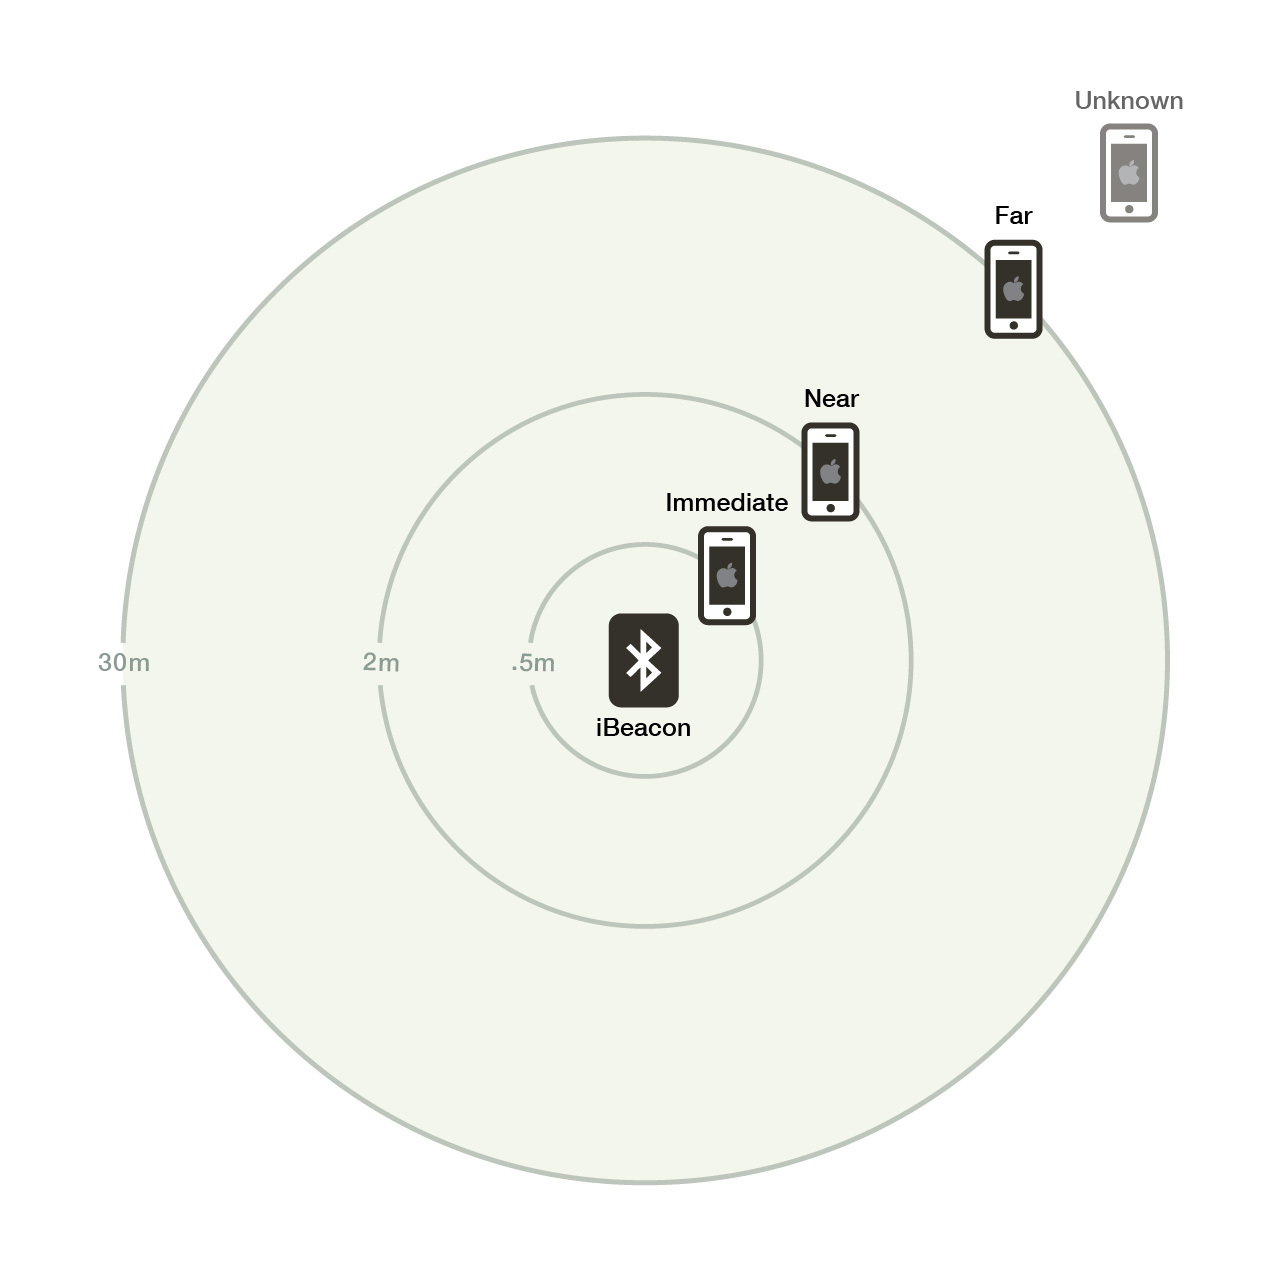
\includegraphics[height=8cm]{images/ibeacon-distance.jpg}
  \caption{Distance categories for iBeacon}
  \label{fig:ibeacon}
\end{figure}
\vspace{0.5cm}


In fact, nothing is stopping this technology from being squeezed into something as small as a typical credit card, or from being embedded in any clothing or other discrete wearable devices such fitness sensors, wristwatches or even temporary tattoos. The opportunities are indeed countless.
Whether we wear those sensors or use them in our homes and businesses (see smart thermostats, lighting and security systems for example), they can all be prepared and trained to cooperate in sophisticated and unexpected ways once the Internet knows that we are present nearby and what our intentions might be. Imagine a smart home capable of knowing when we wake up based on the activity monitor on our wrist and begin warming up the house, brewing a pot of coffee and switching off the security system. 
It is evident that with such a capacity for sensing and responding to our needs,  the Internet of things is slowly shaping a brand new world capable of being alive in ways that it has never been before.


\vspace{0.5cm}
\begin{figure}[htbp]
  \centering
    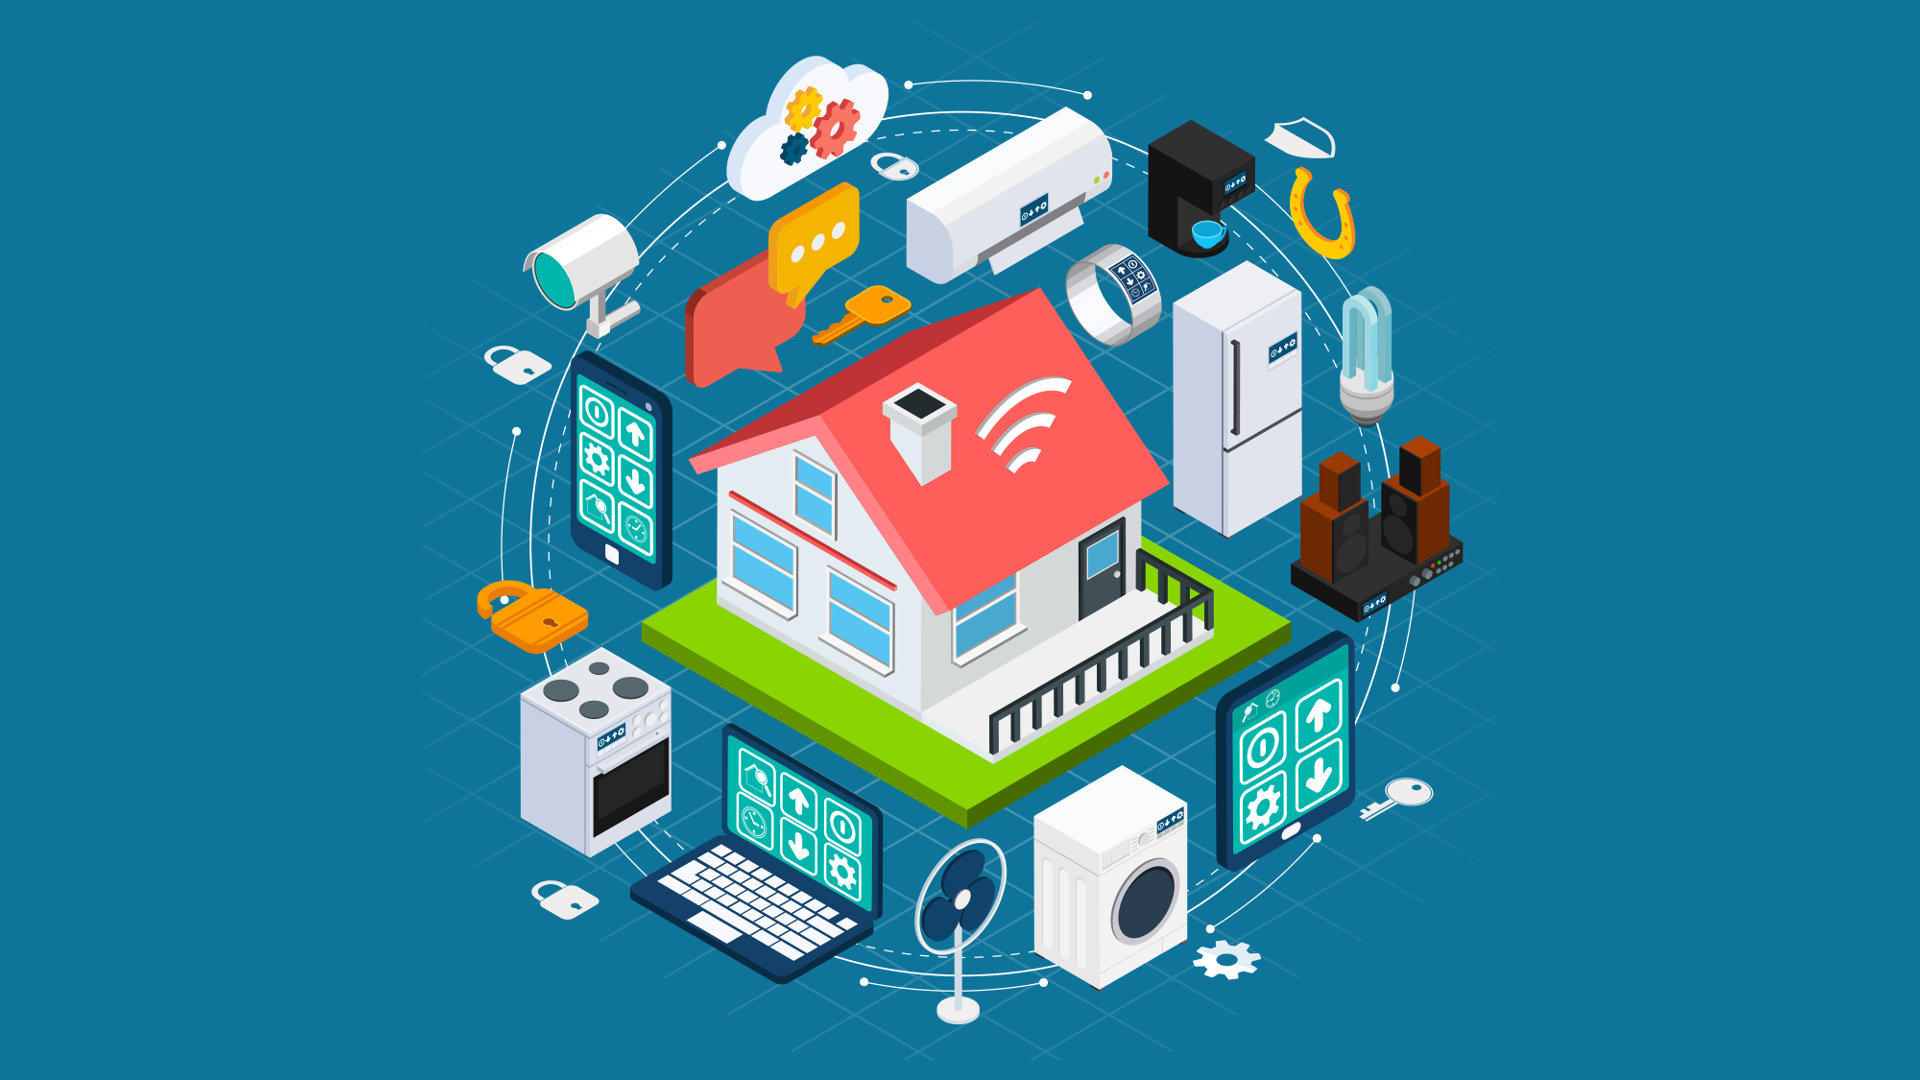
\includegraphics[height=8cm]{images/iot}
  \caption{A smart home ecosystem}
  \label{fig:iot}
\end{figure}
\vspace{0.5cm}

\section{Data and web mining}
\label{section:data-web-mining}
Very often, company management requires selecting the most adequate Business Intelligence solutions that will fit its needs in order to perform crucial strategic decisions.

One of the tools used for this particular goal is a technique called data mining, which is the result of a continuous evolution that has been occuring during the last thirty years of data review.
Up until the late 1970s, Business Intelligence decisions carried out their role through the use of standardized reports which contained simple summarized data and analysis.

In the early 1980s, companies began to query data in more detailed and complex ways. This made it easier to detect patterns based, for example, on an individual product or geographic area.

Currently, the advanced software available on the market for data mining is capable of performing real time pattern detection on a vast quantity of data thrown at it. This expedites a company’s decision making processes and the creation of robust long-term strategies.

\vspace{0.5cm}
\begin{figure}[htbp]
  \centering
    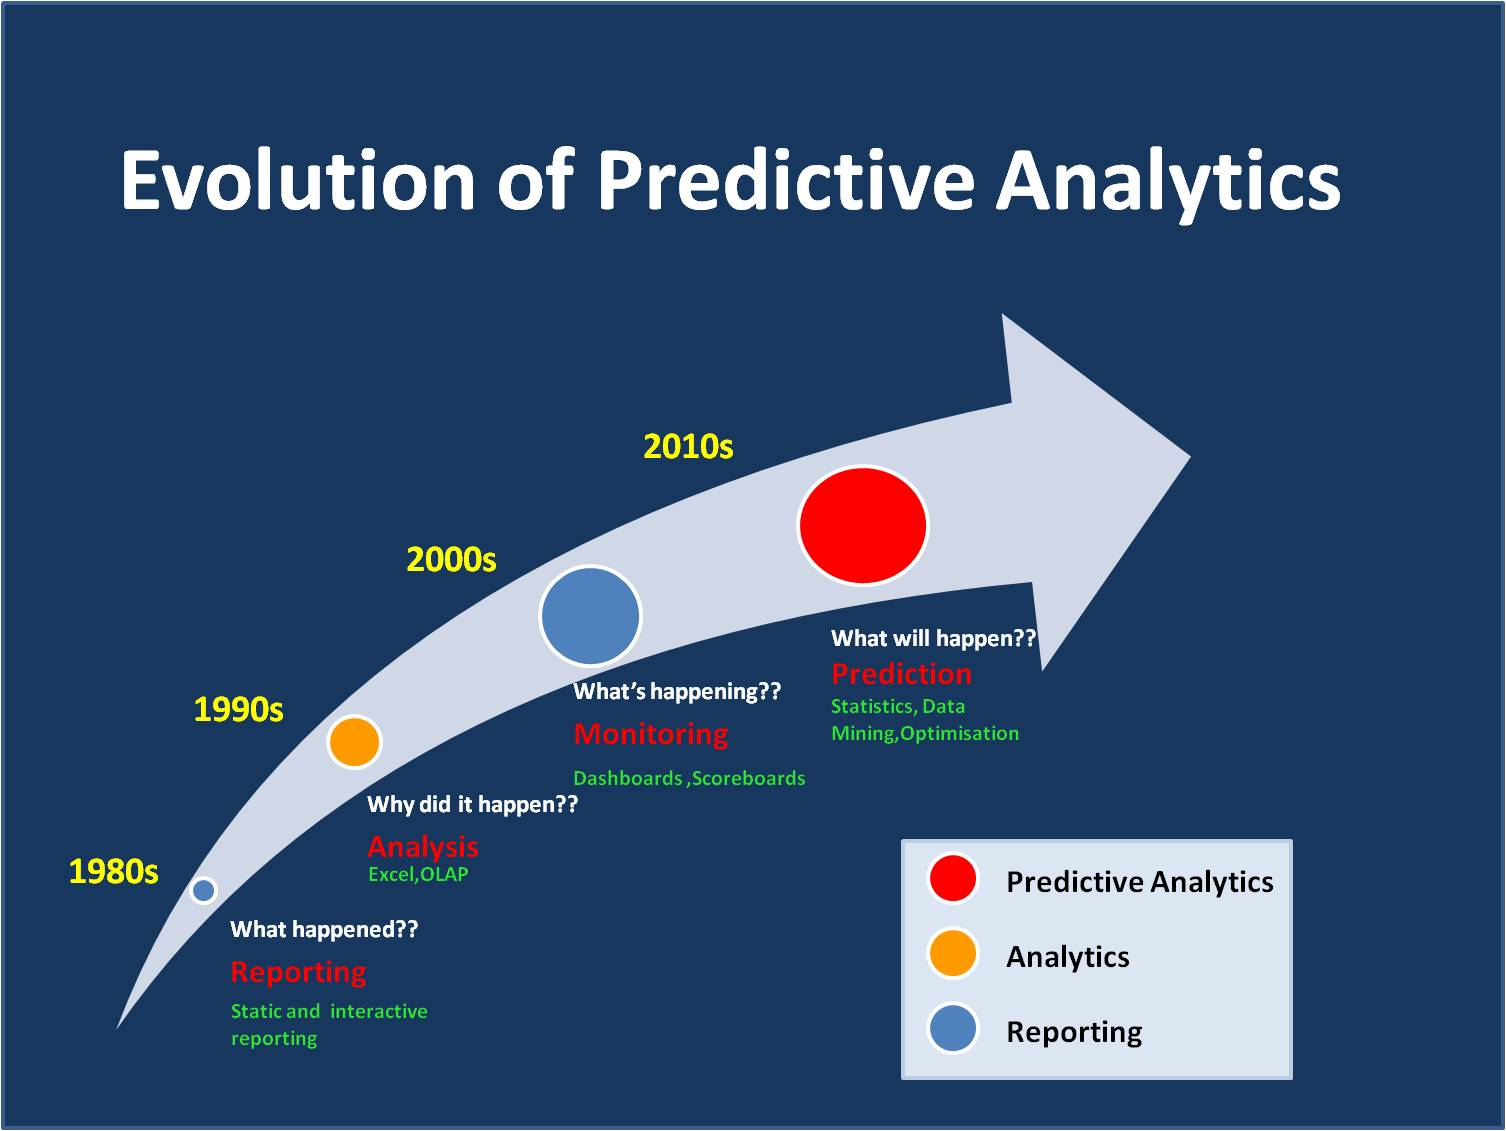
\includegraphics[height=8cm]{images/evolution}
  \caption{Evolution of Predictive Analysis over the last 40 years}
  \label{fig:predict}
\end{figure}
\vspace{0.5cm}
 

Thorough interpretation and analysis of the available data allos the data mining process to create a better overall understanding, and helps in making better decisions.

In fact, thanks to advanced examination techniques, it is possible to find hidden information, create analytical models and data groups, and identify relationships among activities while also correcting errors.

All of this certainly leads to real advantages for a company leveraging these processes, both in terms of revenue and cost. For example, on the side of income, data mining allows companies to identify and classify the best, real and potential customers, discover additional sales opportunities, increase economic productivity and find new ways and new solutions to grow. In parallel, regarding the aspect of cost, the process could maintain clientele by identifying customer loyalty elements, reducing exposure to non-payment risks and distributing resources more efficiently.

For an organization, the reasons behind using data mining may be different.
The unifying point, however, is the need to derive insight from the data that will guide the transformation, reorganization or innovation of business processes.
It is evident that decisions based on accurate and reliable knowledge are always the best. Data mining, in fact, provides exactly this type of information.
While Enterprise Resource Planning (ERP) systems improve operational efficiency, they do not provide the strategic drive for business growth or business change. Warehousing systems can efficiently store data, but they lack the tools to transform those figures into valuable information focused on reporting and answering mostly static questions such as areas where the company has sold the most. On the other side, data mining tools try to present a solution to a wider range of more interesting problems, such as why sales are not taking off as expected, why customers prefer competitors or which previous marketing campaigns had the best outcomes.

Understanding the answers to these questions means taking the right measures to improve the business’s performance.

Besides data visualization techniques, one of the most popular data mining processes on the market is based on the simplified transposition of the neural networks and the neural process of the human brain: when presented with models, the brain understands that some patterns are associated with other desired results. Similarly, artificial neural networks are capable, by learning about sets of historical data called learning sets, to generate patterns and validate them on other subsets of data called test sets. They operate iteratively by modifying patterns from time to time to reach an optimal solution, and they have the ability to evaluate and provide feedback on unknown data, thus making them very useful for forecasting and classifying knowledge. They are very often presented as a "black box" approach to data mining, and they turn out to be very useful when creating parametric models that are difficult to construct and when the emphasis is on forecasting rather than explaining complex patterns.


\vspace{0.5cm}
\begin{figure}[htbp]
  \centering
    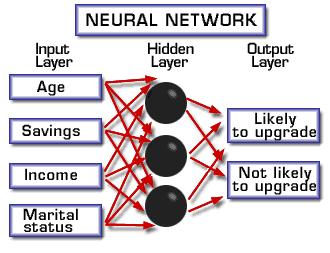
\includegraphics[height=5cm]{images/neural}
  \caption{Neural networks learn to predict outputs after proper training and weighting.}
  \label{fig:neural}
\end{figure}
\vspace{0.5cm}

After discovering what data mining means, who uses it the most, and how it is usually implemented, it is important to focus our attention on the utilization of this tool on the web and its characteristics in such an environment.

In fact, web data mining can detect behavioral models of website visitors, generate reports and implement actions based on those identified patterns.
This process is possible because website visitors often unknowingly provide information about themselves and how they respond to the content presented. Monitoring what links they click, where most of their time is spent, what search terms are entered and when the visitors leave the website are just a few appetizers of the endless stream of possible data inputs.

Some visitors also provide information about their lifestyle or personal information such as names and addresses.

Because of all of this, a thorough and adaptive analysis of this considerable amount of stored information is fundamental, and this is exactly where web data mining kicks in by helping to design the web shopper behavioral model and making valuable predictions.

One of the features that unquestionably contributes to the strength of data mining is the ability to combine emerging traffic data to the site with those related to the transactions and the profile of the buyers.

Through these combinations and by highlighting the patterns that are uncovered, it is possible to both gather complex and strategic considerations and generate predictions that may be indispensable and vital for managing a website that wants to improve its business.

\vspace{0.5cm}
\begin{figure}[!htbp]
  \centering
    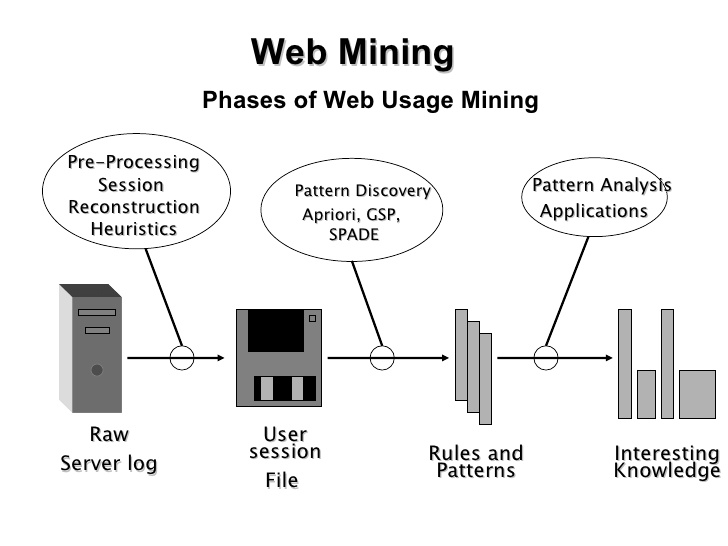
\includegraphics[height=8cm]{images/webmining}
  \caption{Phases of Web Usage Mining}
  \label{fig:webmining}
\end{figure}
\vspace{0.5cm}

Due to the heterogeneity nature of the source data, Web Mining is far from simply being an application of traditional data mining techniques. In fact, it can be categorized into three main types:

\begin{itemize}
  \item \textbf{Web structure mining}:  This focuses on analyzing and discovering useful knowledge from hyperlinks representing the structure of the Web. For example, these links allow us to detect relevant Web pages in a way similar to what search engines are already doing. Alternatively, it is possible to determine shared common interests among users and so on.
  \item \textbf{Web content mining}: The main goal of this technique is to extract valuable information or data from the content of the web pages. After doing so, it is possible to automatically classify and group this information according to topic area. While these tasks are apparently similar to those in traditional data mining, we still can discover relevant behavioral models using product descriptions, forum posts, customer reviews and much more.
  \item \textbf{Web usage mining}: This technique usually refers to the identification of user access patterns from Web usage logs once the sanitization and preprocessing of the clickstream data has occurred.
\end{itemize} 



Although the web mining process is similar to traditional data mining techniques, the data gets collected in an entirely different way. In traditional data mining, the data is often already available and stored in a data warehouse, whereas for the web counterpart, the effort for the data acquisition can be a cumbersome task, especially for web structure and content mining. This is due to the potentially high number of links and large quantity of pages to crawl.

\section{Model-driven techniques}
\label{model-driven-techniques}
Software development techniques are continuously evolving while also trying to solve the principal problems that still affect the building and maintenance of software: time, costs and susceptability to errors.

On this topic, one of the latest research trends in software engineering is the Model Driven Engineering (MDE) technique, which was born as an extension of more specific approaches such as the Model-Driven Architecture (MDA) of the Object Management Group (OMG).\footnote{The Object Management Group (OMG) is an international, open membership, not-for-profit technology standards consortium, founded in 1989. OMG standards are driven by vendors, end-users, academic institutions and government agencies. } 

MDE's primary goal is to define the methodologies and techniques to support the process related to the entire lifecycle of software development through the manipulation of models.

Before proceeding further, it is beneficial to explain the difference between MDA, Model-Driven Development (MDD), MDE and Model-Based Engineering (MBE).

The first is, by all means, an OMG standard focused on software development and using a set of defined languages utilized for a specific purpose (e.g. UML\footnote{The Unified Modeling Language (UML) is a general-purpose, developmental, modeling language in the field of software engineering, that is intended to provide a standard way to visualize the design of a system.}). On the other hand, the focus of MDD is still on software development, but is independent of mandatory language constraints to perform its tasks.
MDE, as a superset of MDD, does not only drop the software-related restrictions, but it unties itself from a particular development process, therefore expediting the definition of model driven processes to facilitate a complete software engineering process. 
Finally, we use MBE to refer to a softer version and a superset of MDE where models still play an important role, but are not the central artifacts of the development process. (e.g. blueprints or sketches of the system handed out to programmers directly without automatic code generation) ( Figure \ref{fig:mda} ).

\vspace{0cm}
\begin{figure}[htbp]
  \centering
    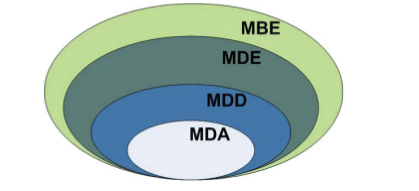
\includegraphics[height=4cm]{images/mda}
  \caption{Relationship between the different MD* acronyms.}
  \label{fig:mda}
\end{figure}
\vspace{0cm}

The model is at the center of any MDE process and, to be considered as such, the modeling language that generated it needs to have well-formalized syntax and semantics. This is a fundamental condition for the automatic transformation of models. In fact, the model represents the system and constitutes an abstract and conforming formalization to a particular language. Such a language is often tailored to a certain domain and is often called Domain-Specific Language (DSL). 

The advantages of using the model driven approach rely on the consideration of the generating language as a type of scheme that is also fully modelable through a formal and abstract definition known as the meta-model. In fact, the model must represent an abstraction of the concepts of the system that needs to be built, while also respecting a meta-model likewise determined by the application domain.

This reasoning can be further iterated up to the determination of a model for the representation of languages used to formalize other languages (the meta-meta model).

Because of the above, model-driven approaches are often defined by models on a stack basis as shown on Figure \ref{fig:mde}.

\vspace{0cm}
\begin{figure}[htbp]
  \centering
    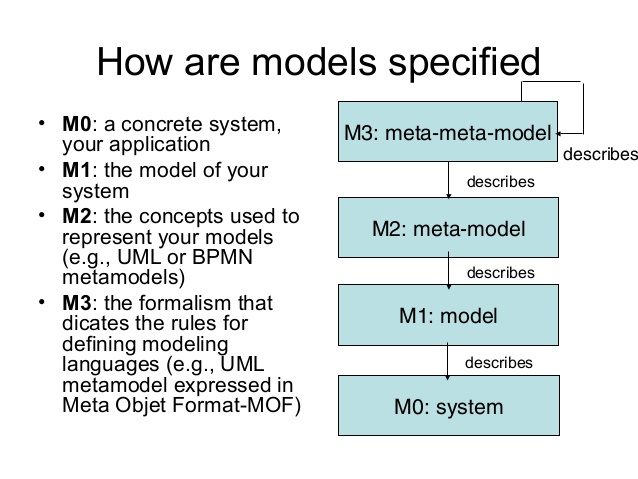
\includegraphics[height=8cm]{images/mde}
  \caption{Models stack}
  \label{fig:mde}
\end{figure}
\vspace{0cm}

One of the most commonly used techniques in MDE is the automatic model generation based on the definition of a set of automatic transformations defined by the starting and target languages. In a nutshell, the MDE approach consists of:

\begin{itemize}
  \item \textbf{Models Generation}, based on modeling stacks definition supporting meta-modelling methods where lower-level models comply with what is specified by higher-level models.

  \item \textbf{Models Manipulation} performed through transformations expected to generate destination models which conform to destination meta-models when provided with source models that conform to source meta-models.
\end{itemize} 

In summary, MDE techniques allow, on the one hand, for the management of the complexity of a system by ensuring increased productivity, and for quality improvements by promoting a higher level of abstraction and reuse, on the other. This result is achieved through a process of engineering, both for the languages and the transformations involved: they are, in fact, the basis of a system’s development process because they represent the transition from higher-level models into lower-level ones until they can be made executable using either automatic code generation or model interpretation.

%\addcontentsline{toc}{chapter}{}

